\documentclass[12pt, a4paper]{article}

\usepackage[utf8]{inputenc}
\usepackage[T1]{fontenc}
\usepackage{amsmath}
\usepackage{graphicx}
\usepackage[colorlinks=true, allcolors=blue]{hyperref}
\usepackage[numbers,sort&compress]{natbib}
\usepackage{geometry}
\usepackage{caption}
\usepackage{fancyhdr}
\usepackage{booktabs}
\usepackage{amssymb}
\usepackage{amsfonts}

\geometry{a4paper, margin=1in}
\setlength{\headheight}{14.5pt}
\pagestyle{fancy}
\fancyhf{}
\rhead{Spatial Audio Feature Extraction}
\lhead{Methodology Report}
\cfoot{\thepage}

\title{A Methodological Framework for Extracting and Visualizing Spatial Audio Features from Binaural Recordings}
\author{Douglas Abreu}
\date{\today}

\begin{document}

\maketitle

\begin{abstract}
\noindent This report provides a comprehensive scientific description of a software framework designed for the analysis of spatial audio. The core methodology revolves around the extraction of a rich set of binaural and spatial features from stereo audio recordings, which are subsequently visualized as composite image mosaics. This process facilitates the analysis of spatial characteristics and prepares the data for application in machine learning models. The pipeline begins with standardized audio preprocessing, including loudness normalization based on the ITU-R BS.1770-4 standard. A multi-resolution Short-Time Fourier Transform (STFT) analysis is then employed to capture both transient and stationary signal characteristics. From this time-frequency representation, a suite of key spatial features is computed, including Interaural Level Difference (ILD), Interaural Phase Difference (IPD), Interaural Cross-Correlation (IACC), and Magnitude-Squared Coherence (MSC). Interaural Time Difference (ITD) is robustly estimated using the Generalized Cross-Correlation with Phase Transform (GCC-PHAT) algorithm. Spectrograms are enhanced using Per-Channel Energy Normalization (PCEN) to improve signal robustness. Finally, these feature maps are systematically arranged into a standardized mosaic image, providing a holistic and visually coherent representation of the audio's spatial properties. This work establishes a reproducible and extensible methodology for computational spatial audio analysis.
\end{abstract}

\section{Introduction}

The ability of the human auditory system to localize sound sources in three-dimensional space is a remarkable feat of neural processing. This capability, known as spatial hearing, relies primarily on the subtle differences between the signals received at the two ears \cite{blauert1997spatial}. These differences, or binaural cues, provide the brain with the necessary information to perceive the direction and distance of a sound source. The computational modeling and analysis of these cues are fundamental to a wide range of audio technologies, from immersive virtual reality and hearing aids to automatic format classification and scene analysis.

This report details the methodology of a software system designed to automate the extraction and visualization of these critical spatial audio features. The primary goal of the framework is to convert a binaural or stereo audio recording into a compact and informative image-based representation. This ``spatial mosaic'' encapsulates a wide array of features that describe the spatial characteristics of the audio signal over time and frequency. Such a representation is not only useful for human-led analysis and quality assessment but is also specifically designed for ingestion by modern computer vision models, such as Convolutional Neural Networks (CNNs) or Vision Transformers (ViTs), enabling the application of powerful machine learning techniques to tasks in spatial audio.

The methodology is divided into three main stages: (1) a rigorous preprocessing and normalization stage to ensure signal consistency; (2) a comprehensive feature extraction stage where a variety of established spatial cues are computed using a multi-resolution time-frequency analysis; and (3) a visualization stage where these features are normalized and arranged into a standardized mosaic image. This document provides a detailed, step-by-step explanation of each component, grounded in the relevant scientific literature.

\section{Theoretical Background}

\subsection{Fundamentals of Binaural Hearing}
The perception of sound source location is largely governed by three primary binaural cues. For frequencies below approximately 1.5 kHz, the dominant cue is the \textbf{Interaural Time Difference (ITD)}, which arises from the difference in the path length of the sound wave to the two ears. For higher frequencies, the head casts an "acoustic shadow," creating an \textbf{Interaural Level Difference (ILD)}, which serves as the primary localization cue. A third important cue is the \textbf{Interaural Cross-Correlation (IACC)}, a measure of the similarity of the signals at the two ears, which is related to the sense of spaciousness and envelopment \cite{blauert1997spatial, breebaart2001binaural}. These fundamental cues form the basis for the feature extraction process.

\subsection{Time-Frequency Analysis}
Audio signals are non-stationary, meaning their statistical properties change over time. Therefore, to analyze them effectively, it is necessary to use a time-frequency representation. The \textbf{Short-Time Fourier Transform (STFT)} is a standard method for this purpose. It involves computing the Fourier transform over short, overlapping windows of the signal, yielding a spectrogram that represents the signal's frequency content over time \cite{griffin1984signal}. The choice of window size presents a trade-off: short windows provide good temporal resolution (ideal for transients), while long windows provide good frequency resolution (ideal for stationary sounds). Our methodology addresses this by employing a multi-resolution approach.

\subsection{Loudness Perception}
The perceived loudness of a signal is not directly proportional to its physical amplitude (e.g., RMS level). To account for the characteristics of human hearing, standardized loudness measures have been developed. The \textbf{ITU-R BS.1770} recommendation specifies an algorithm for measuring audio programme loudness and true-peak level, resulting in a value measured in Loudness Units relative to Full Scale (LUFS). This standard incorporates a K-weighting filter to approximate the frequency sensitivity of human hearing \cite{itu2015bs1770}. Standardizing loudness is a critical preprocessing step for any comparative audio analysis.

\section{Methodology}
The software pipeline is a sequential process that transforms a stereo audio file into a feature mosaic image and an accompanying HDF5 data file. The process is deterministic and designed for full reproducibility.

\subsection{Audio Preprocessing and Normalization}
The initial stage ensures that all audio files are processed in a consistent manner, removing variations that are not related to spatial characteristics.
\begin{enumerate}
    \item \textbf{Loading and Resampling:} The input audio file is loaded into memory. To standardize all subsequent frequency-domain calculations, the signal is resampled to a target sampling rate of 48 kHz. The system validates that the input is a stereo file, as binaural features are predicated on a two-channel input.
    \item \textbf{Loudness Normalization:} To ensure perceptual consistency across different audio files, the loudness of each file is normalized. While several methods are available (Peak, RMS), the primary approach utilizes the \textbf{ITU-R BS.1770-4} standard to adjust the signal to a target level of -23.0 LUFS \cite{itu2015bs1770}. This method is preferred as it incorporates a K-weighting filter that approximates the frequency sensitivity of human hearing, thus aligning the normalization with perceptual loudness. The normalization process involves applying a calculated gain to the raw audio waveform. To prevent clipping, a safety mechanism is implemented that limits the applied gain, ensuring the peak level does not exceed a maximum threshold (e.g., 0.99).

    \noindent In order to preserve binaural spatial cues, the implementation favors simple uniform-gain normalizations (RMS/Peak/LUFS) that apply the same scalar gain to all channels. When dynamic range reduction is required, the pipeline uses a \emph{mono-linked soft compression} strategy: the envelope is computed from the mono mix (or the aggregated channel energy) and the same sample-wise gain reduction is applied to every channel. This design choice prevents independent per-channel compression which can alter interaural level differences (ILD) and temporal envelopes important for interaural time difference (ITD) perception.
\end{enumerate}

\subsection{Multi-Resolution Time-Frequency Analysis}
To analyze the non-stationary audio signal, it is first transformed into a time-frequency domain representation using the Short-Time Fourier Transform (STFT). The STFT for a signal $x[n]$ is defined as:
\begin{equation}
    X(t, f) = \sum_{n=-\infty}^{\infty} x[n] w[n-tH] e^{-j2\pi fn}
\end{equation}
where $w[n]$ is a window function and $H$ is the hop size.

To capture a comprehensive view of the signal's characteristics, a multi-resolution analysis is performed on the normalized left ($x_L[n]$) and right ($x_R[n]$) audio channels. This approach addresses the inherent trade-off between time and frequency resolution in STFT analysis.
\begin{itemize}
    \item \textbf{Short-Time Analysis:} A window size of 2048 samples is used to provide high temporal resolution. This is effective for capturing transient events and sharp onsets, which are critical for localization.
    \item \textbf{Long-Time Analysis:} A window size of 4096 samples is used to provide high frequency resolution. This is better suited for analyzing stationary sounds, ambient characteristics, and the diffuse nature of reverberant fields.
\end{itemize}
Both transforms use a Hann window and a 50\% overlap, producing complex-valued spectrograms ($X_L(t,f)$ and $X_R(t,f)$) for each channel at two different resolutions.

\subsection{Spatial Feature Extraction}
From the multi-resolution STFTs, a dictionary of spatial features is computed. These features are designed to explicitly expose the binaural cues that the human auditory system uses for spatial perception.

\begin{description}
    \item[Magnitude Spectrograms with PCEN:] The magnitude of each STFT, $|X(t,f)|$, is taken. To enhance this representation, \textbf{Per-Channel Energy Normalization (PCEN)} is applied. PCEN is a form of adaptive gain control that performs a channel-wise dynamic compression, emphasizing onsets and de-emphasizing stationary components. This makes the representation more robust to variations in recording level and background noise, often outperforming simple logarithmic compression in noisy environments \cite{wang2017per}.
    
    \item[Interaural Level Difference (ILD):] The ILD is a primary cue for localizing sounds in the horizontal plane, especially at high frequencies. It is calculated as the logarithmic ratio of the energy in the left and right channels for each time-frequency bin, expressed in decibels.
    \begin{equation}
        \text{ILD}(t, f) = 20 \log_{10} \left( \frac{|X_L(t, f)|}{|X_R(t, f)| + \epsilon} \right)
    \end{equation}
    where $\epsilon$ is a small constant to prevent division by zero. An ILD of approximately zero is characteristic of a monophonic or central sound source.
    
    \item[Interaural Phase and Time Differences (IPD/ITD):] The IPD captures the phase difference between the two channels, which is the dominant cue for horizontal localization at low frequencies. It is defined as:
    \begin{equation}
        \text{IPD}(t, f) = \angle X_L(t, f) - \angle X_R(t, f)
    \end{equation}
    To avoid discontinuities from phase wrapping, the IPD is decomposed into its sine and cosine components, which are continuous and well-behaved for machine learning models.
    
    For a broadband estimation of the Interaural Time Difference (ITD), the \textbf{Generalized Cross-Correlation with Phase Transform (GCC-PHAT)} method is used. This is a highly robust technique for time delay estimation in noisy and reverberant environments. The GCC-PHAT function is computed as:
    \begin{equation}
        R_{LR}^{\text{PHAT}}(\tau, t) = \mathcal{F}^{-1} \left\{ \frac{X_L(f, t) X_R^*(f, t)}{|X_L(f, t) X_R^*(f, t)|} \right\}
    \end{equation}
    where $\mathcal{F}^{-1}$ denotes the inverse Fourier transform and $*$ denotes the complex conjugate. The phase transform whitens the signal spectra, sharpening the peak in the cross-correlation function. The time delay $\hat{\tau}(t)$ corresponding to the peak of this function provides an estimate of the ITD for that time frame \cite{knapp1976generalized}.
    
    \item[Interaural Cross-Correlation (IACC):] The IACC measures the similarity of the signals at the two ears and is strongly related to the perception of auditory source width and envelopment. It is computed as the normalized cross-correlation between the left and right channel signals within short time windows for each frequency band. A high IACC (close to 1) indicates a narrow, central source (typical of mono), while a low IACC suggests a wide, diffuse sound field (typical of surround sound) \cite{breebaart2001binaural}.
    
    \item[Magnitude-Squared Coherence (MSC):] MSC is a frequency-domain measure of the linear relationship between the two channels. It is calculated from the cross-power spectral density ($P_{LR}$) and the auto-power spectral densities ($P_{LL}$, $P_{RR}$):
    \begin{equation}
        C_{LR}(t, f) = \frac{|P_{LR}(t, f)|^2}{P_{LL}(t, f) P_{RR}(t, f)}
    \end{equation}
    Like IACC, coherence values close to 1 indicate a strong relationship (mono/central source), while lower values are characteristic of reverberant or multi-source environments.
    
    \item[Mid/Side Decomposition:] The left/right signals are converted to Mid ($M$) and Side ($S$) components, which separate the common and differential information, respectively.
    \begin{align}
        M(t, f) &= \frac{X_L(t, f) + X_R(t, f)}{2} \\
        S(t, f) &= \frac{X_L(t, f) - X_R(t, f)}{2}
    \end{align}
    Spectrograms of the Mid and Side components are generated, along with a \textit{laterality index} $\rho(t, f) = |S(t,f)| / (|M(t,f)| + \epsilon)$, which highlights the proportion of side-channel energy. Monophonic content has a low laterality index.
    
    \item[Spectral Features for Elevation Cues:] The direction-dependent filtering of the outer ear (pinna) creates notches in the high-frequency spectrum of incoming sounds, which are important cues for elevation. To capture these effects, spectral features such as the \textbf{spectral centroid} and \textbf{spectral slope} are computed for each channel. These features describe the "brightness" and tilt of the spectrum and can help distinguish sounds with significant overhead content (e.g., 5.1+4h) \cite{jehan2005creating}.
\end{description}

\subsection{Mosaic Image Generation}
The final stage of the pipeline is the creation of a standardized visual representation of the extracted features.
\begin{enumerate}
    \item \textbf{Feature Normalization:} Each feature map is normalized to an appropriate range for visualization. For example, IACC and IPD components are mapped to the [0, 1] range, while ILD is clipped to a perceptually relevant range (e.g., $\pm$20 dB) before normalization.
    \item \textbf{Resizing:} All feature maps are resized to a consistent dimension (e.g., 128x200 pixels) using an anti-aliasing filter to ensure uniformity.
    \item \textbf{Mosaic Assembly:} The resized feature maps are arranged in a predefined 4$\times$6 grid. A \texttt{viridis} colormap is applied to convert the single-channel, normalized feature maps into RGB representations. Text labels are added to each block to identify the feature.
    \item \textbf{Final Image Creation and Saving:} The assembled mosaic is resized to a final target dimension (e.g., 512x512 pixels). The resulting image is saved in a standard format (e.g., PNG or TIFF).
    \item \textbf{Raw Data Archiving:} In parallel, the raw, unprocessed dictionary of features is saved to an HDF5 file. This ensures that the full-precision numerical data is preserved for future analysis, allowing for complete reproducibility of the results.
\end{enumerate}

% --- Detailed mosaic description and example figures inserted below ---
\subsubsection{Detailed Mosaic Layout and Interpretation}
The mosaic image is constructed as a regular grid of feature blocks arranged in a 4$\times$6 layout (rows $\times$ columns), producing 24 individual tiles. Each tile corresponds to a single-channel feature map computed from the multi-resolution STFT analysis and subsequent processing stages. Feature maps are normalized to an appropriate visualization range, resized to a uniform block dimension (e.g., 128$\times$200 pixels), and mapped to RGB using the \texttt{viridis} colormap to enhance perceptual contrast while preserving relative magnitude information.

For reproducibility and to support downstream machine learning tasks, the canonical order of features in the mosaic is fixed. The order (left-to-right, top-to-bottom) and their short labels are as follows:
\begin{center}
\begin{tabular}{ll}
1. Mag L (S) & 13. Mid (S) \\
2. Mag R (S) & 14. Side (S) \\
3. ILD (S) & 15. Lat (S) \\
4. IPD Sin (S) & 16. Mid (L) \\
5. IPD Cos (S) & 17. Side (L) \\
6. IACC (S) & 18. Lat (L) \\
7. Mag L (L) & 19. MSC (S) \\
8. Mag R (L) & 20. MSC (L) \\
9. ILD (L) & 21. GCC-PHAT \\
10. IPD Sin (L) & 22. SC L (S) \\
11. IPD Cos (L) & 23. SS L (S) \\
12. IACC (L) & 24. Late E (S) \\
\end{tabular}
\end{center}

Each entry above has a specific interpretative role:
\begin{itemize}
    \item \textbf{Magnitude (Mag L/R)}: PCEN-enhanced magnitude spectrograms for left and right channels at short (S) and long (L) resolutions. Short-resolution blocks emphasize transient events; long-resolution blocks emphasize stationary spectral structure.
    \item \textbf{ILD (Interaural Level Difference)}: Encodes level differences between channels per time-frequency bin; clipped to a perceptual range (e.g., $\pm$20 dB) to highlight lateralization without saturating visualization.
    \item \textbf{IPD (Interaural Phase Difference) -- Sin/Cos}: Phase difference decomposed into sine and cosine components to avoid phase-wrapping discontinuities; useful for models to learn angular cues continuously.
    \item \textbf{IACC (Interaural Cross-Correlation)}: Short/long-window estimates of signal similarity across ears; high values indicate a compact, central source while low values indicate diffuse or reverberant fields.
    \item \textbf{Mid/Side and Laterality}: Mid (M) and Side (S) spectrograms separate common and differential content; laterality index highlights the relative contribution of side energy, discriminating center vs lateralized sources.
    \item \textbf{MSC (Magnitude-Squared Coherence)}: Bandwise coherence between channels, complementary to IACC; near-unity values indicate strong linear relation across channels.
    \item \textbf{GCC-PHAT}: Time-delay correlation map (PHAT weighting) providing robust broadband ITD cues; peaks correspond to candidate interaural time differences.
    \item \textbf{Spectral Centroid / Slope / Late Energy}: Compact spectral descriptors sensitive to elevation-related filtering and reverberant tail energy respectively.
\end{itemize}

\subsubsection{Visualization and Practical Interpretation}
The mosaic is intended to be simultaneously interpretable by researchers and ingestible by convolutional models. Visual patterns to inspect include:
\begin{itemize}
    \item \textbf{Consistent diagonal/horizontal bands in magnitude tiles}: indicate harmonic structure or stationary tonal content.
    \item \textbf{Strong localized ILD / IPD structure}: suggests clear lateralization of sources; symmetric ILD/IPD around zero suggests central sources.
    \item \textbf{High MSC / IACC across bands}: typically observed for monophonic or single-source recordings; lower coherence across frequencies indicates diffuse or multi-source scenes.
    \item \textbf{Prominent peak in GCC-PHAT tile}: corresponds to a stable ITD estimate; spread or multimodal peaks indicate reverberation or multiple concurrent sources.
\end{itemize}

\subsubsection{Example Mosaic Images}
The following figures show representative mosaic images generated by the pipeline from the dataset class \texttt{514}. These examples illustrate typical patterns described above and facilitate comparison between recordings.

\begin{figure}[h!]
    \centering
    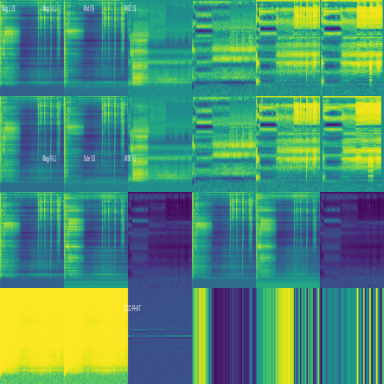
\includegraphics[width=0.32\textwidth]{img/binaural_audio_D1_48K_24bit_0.3s_FIR_SOFA_ac06-globo-1_0_chunk0005.png}
    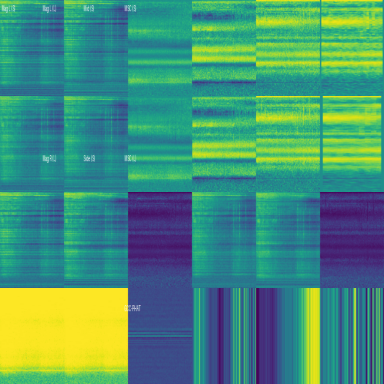
\includegraphics[width=0.32\textwidth]{img/binaural_audio_D1_48K_24bit_0.3s_FIR_SOFA_ac06-globo-1_0_chunk0014.png}
    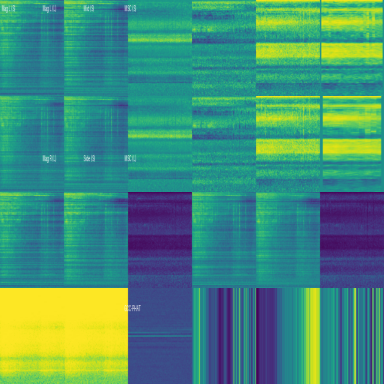
\includegraphics[width=0.32\textwidth]{img/binaural_audio_D2_48K_24bit_0.3s_FIR_SOFA_ac06-globo-1_0_chunk0014.png}
    \caption{Representative mosaic images (class 514). Left: chunk0005; center: chunk0014 (D1); right: chunk0014 (D2). Each mosaic is a 4$\times$6 arrangement of spatial features: magnitude, ILD, IPD, IACC, MSC, GCC-PHAT and spectral descriptors as described in the text.}
    \label{fig:example_mosaics}
\end{figure}

% End insertion

\section{Experimental Analysis and Results}
An analysis was performed on a dataset of 10,935 audio files, totaling 30.38 hours, to evaluate the audio characteristics and the effectiveness of the normalization process. The dataset is categorized into four classes corresponding to the original collection labels: \texttt{100}, \texttt{200}, \texttt{510}, and \texttt{514}. This empirical evaluation validates the necessity of the preprocessing stages.

\subsection{Dataset Audio Characteristics}
The original audio files exhibited a wide range of loudness levels, as summarized in Table \ref{tab:class_summary}. The mean LUFS for the entire dataset was -35.50, with a standard deviation of 5.66 LUFS, indicating variation in perceived loudness that benefits from standardized normalization. This highlights the critical need for a consistent normalization strategy before feature extraction can be reliably performed.

\begin{table}[h!]
\centering
\caption{Summary of Original Audio Characteristics by Class}
\label{tab:class_summary}
\begin{tabular}{@{}lcccc@{}}
\toprule
\textbf{Class Name} & \textbf{Files} & \textbf{Original RMS (dB)} & \textbf{Original Peak (dB)} & \textbf{Original LUFS} \\ \midrule
100 & 2366 & -25.56 $\pm$ 12.34 & -3.48 $\pm$ 14.33 & -35.13 $\pm$ 5.88 \\
200 & 2368 & -25.84 $\pm$ 12.37 & -3.43 $\pm$ 14.33 & -36.60 $\pm$ 5.79 \\
510 & 1873 & -23.91 $\pm$ 2.15 & -3.09 $\pm$ 2.57 & -35.07 $\pm$ 4.01 \\
514 & 4328 & -23.69 $\pm$ 2.25 & -4.30 $\pm$ 2.94 & -35.29 $\pm$ 6.00 \\ \bottomrule
\end{tabular}
\end{table}

\subsection{Normalization Effectiveness}
The LUFS normalization method was applied to standardize the audio levels to a target of -23.0 LUFS. Figure \ref{fig:level_distributions} illustrates the distribution of RMS, Peak, and LUFS levels across the entire dataset before and after normalization. The post-normalization distributions are visibly more concentrated around their target values, demonstrating a significant reduction in level variance.

\begin{figure}[h!]
    \centering
    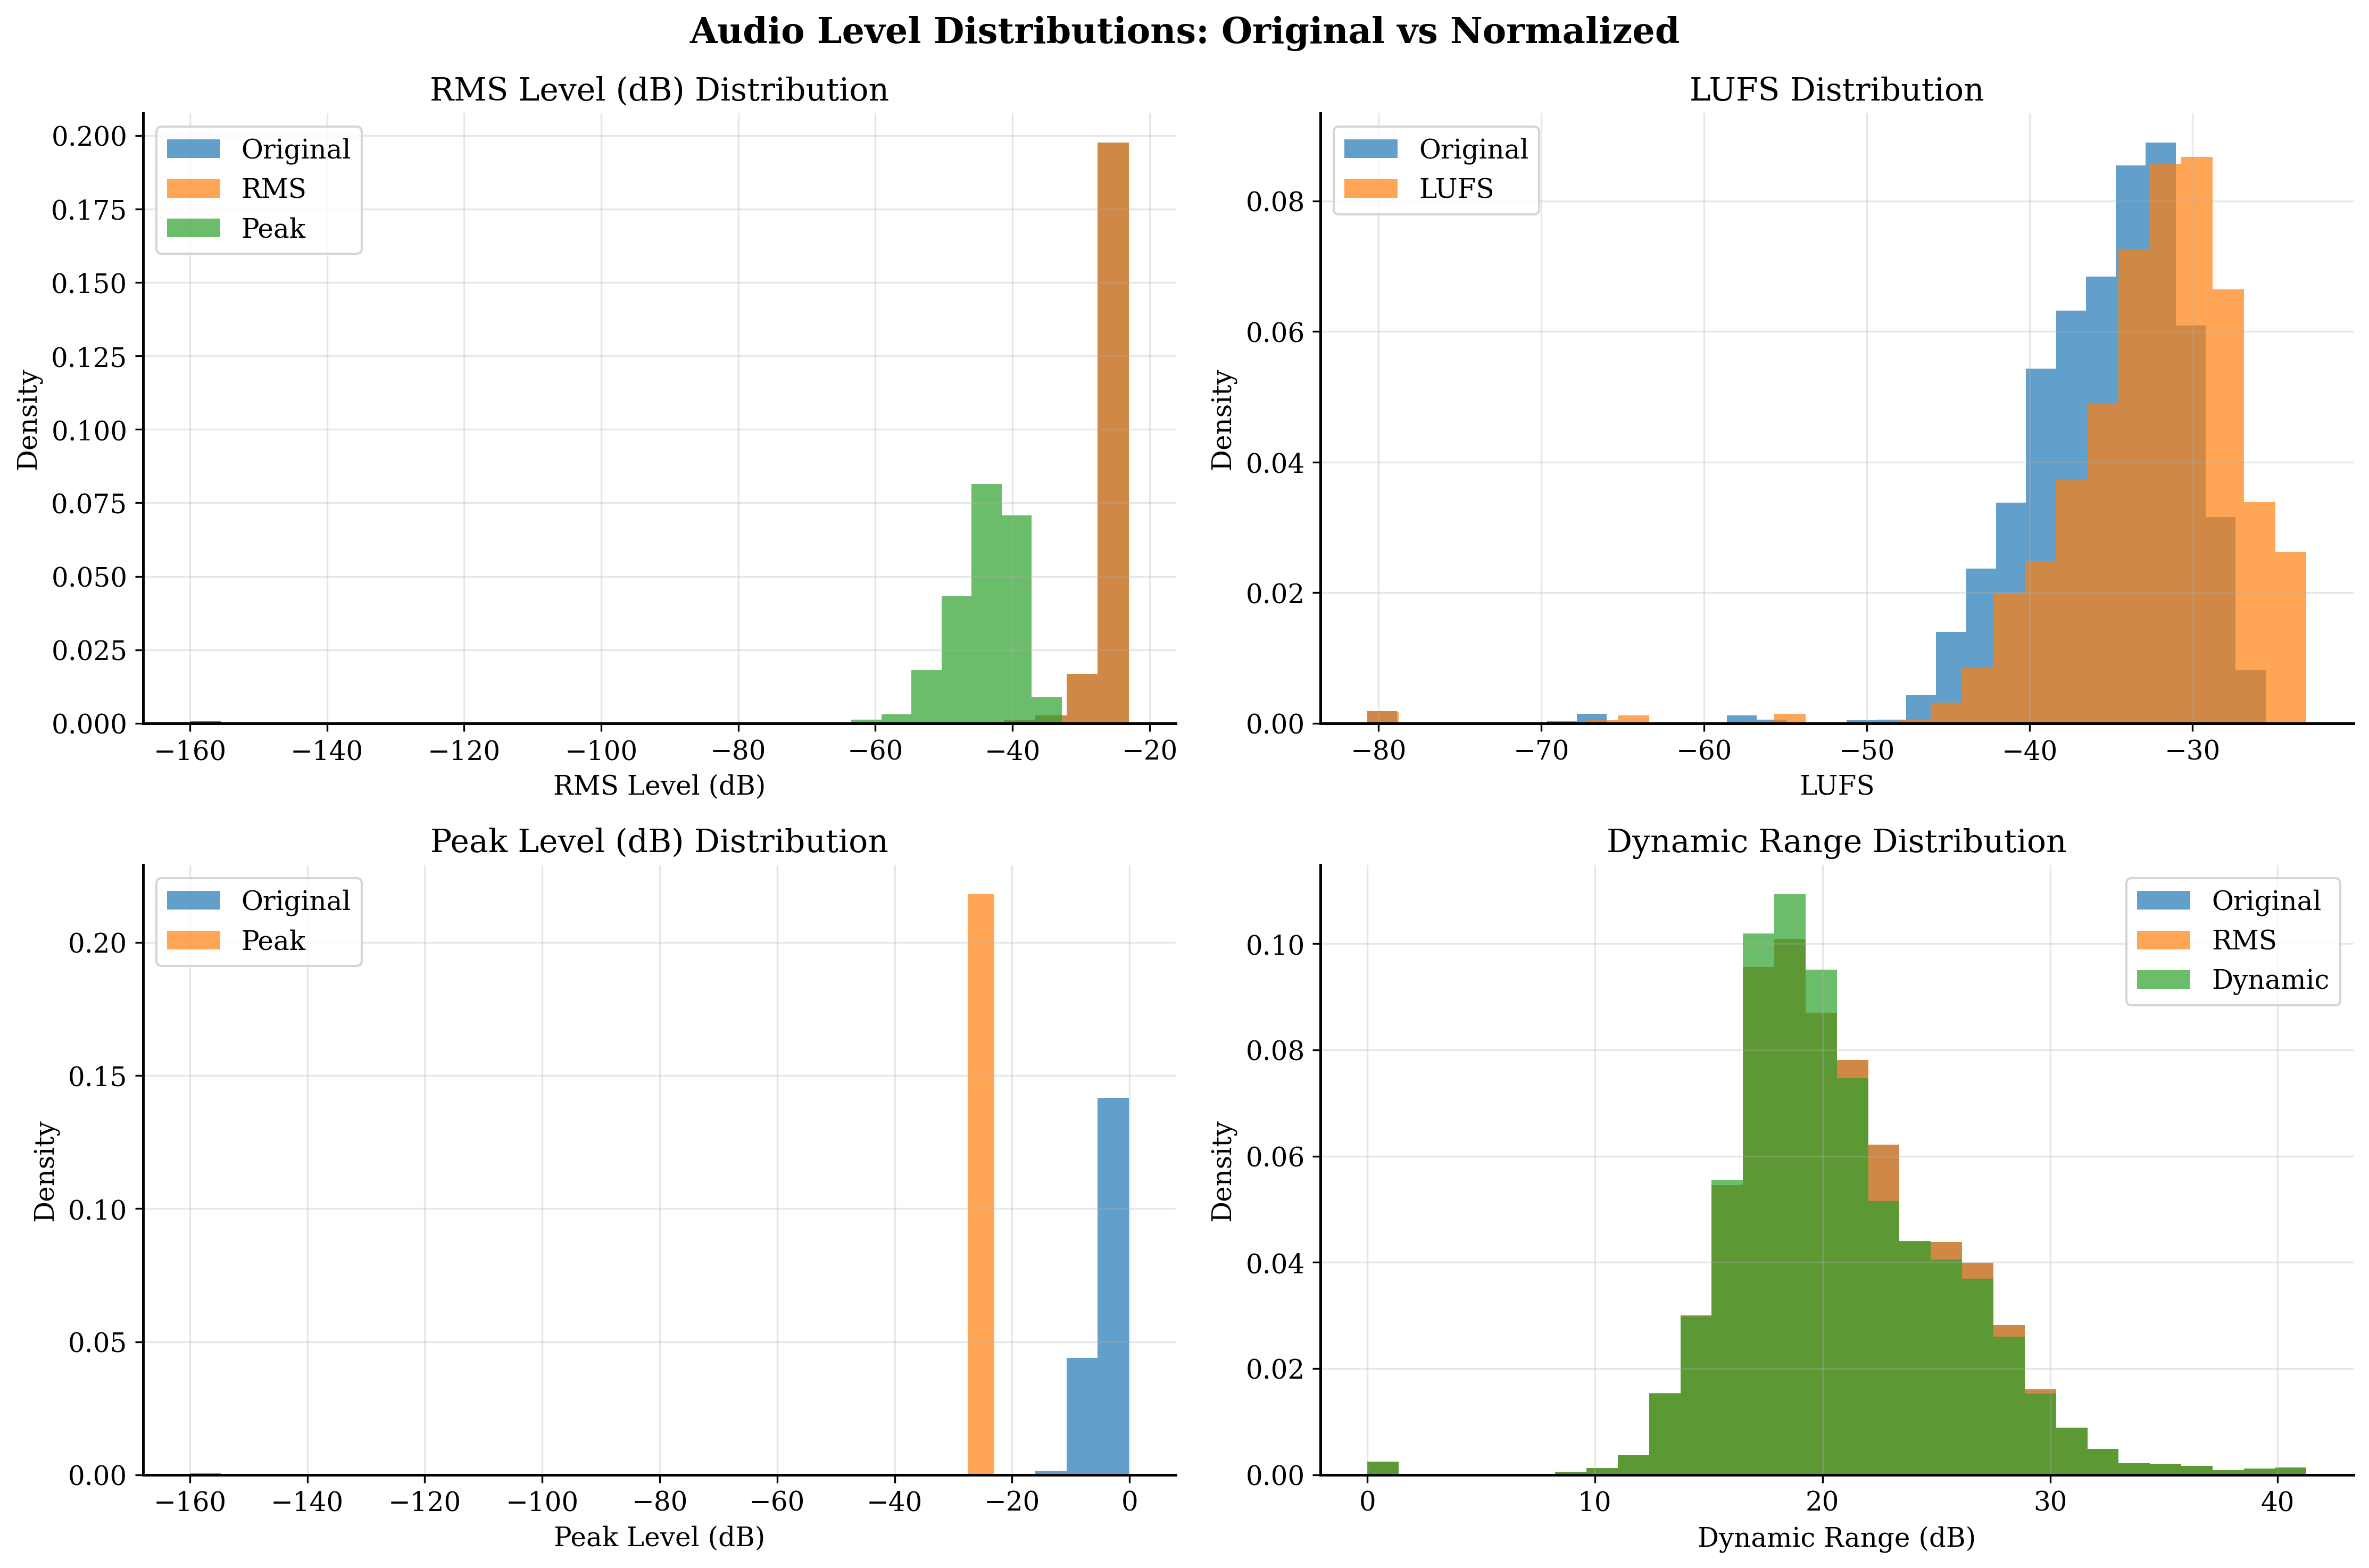
\includegraphics[width=\textwidth]{img/level_distributions.png}
    \caption{Distribution of audio levels (RMS, Peak, and LUFS) before and after normalization across the entire dataset.}
    \label{fig:level_distributions}
\end{figure}

To further quantify the impact of normalization, Figure \ref{fig:norm_effectiveness} provides a comparative visualization. The boxplots clearly show that the range and variance of LUFS values are dramatically reduced after normalization, confirming the effectiveness of the procedure in creating a perceptually consistent dataset.

\begin{figure}[h!]
    \centering
    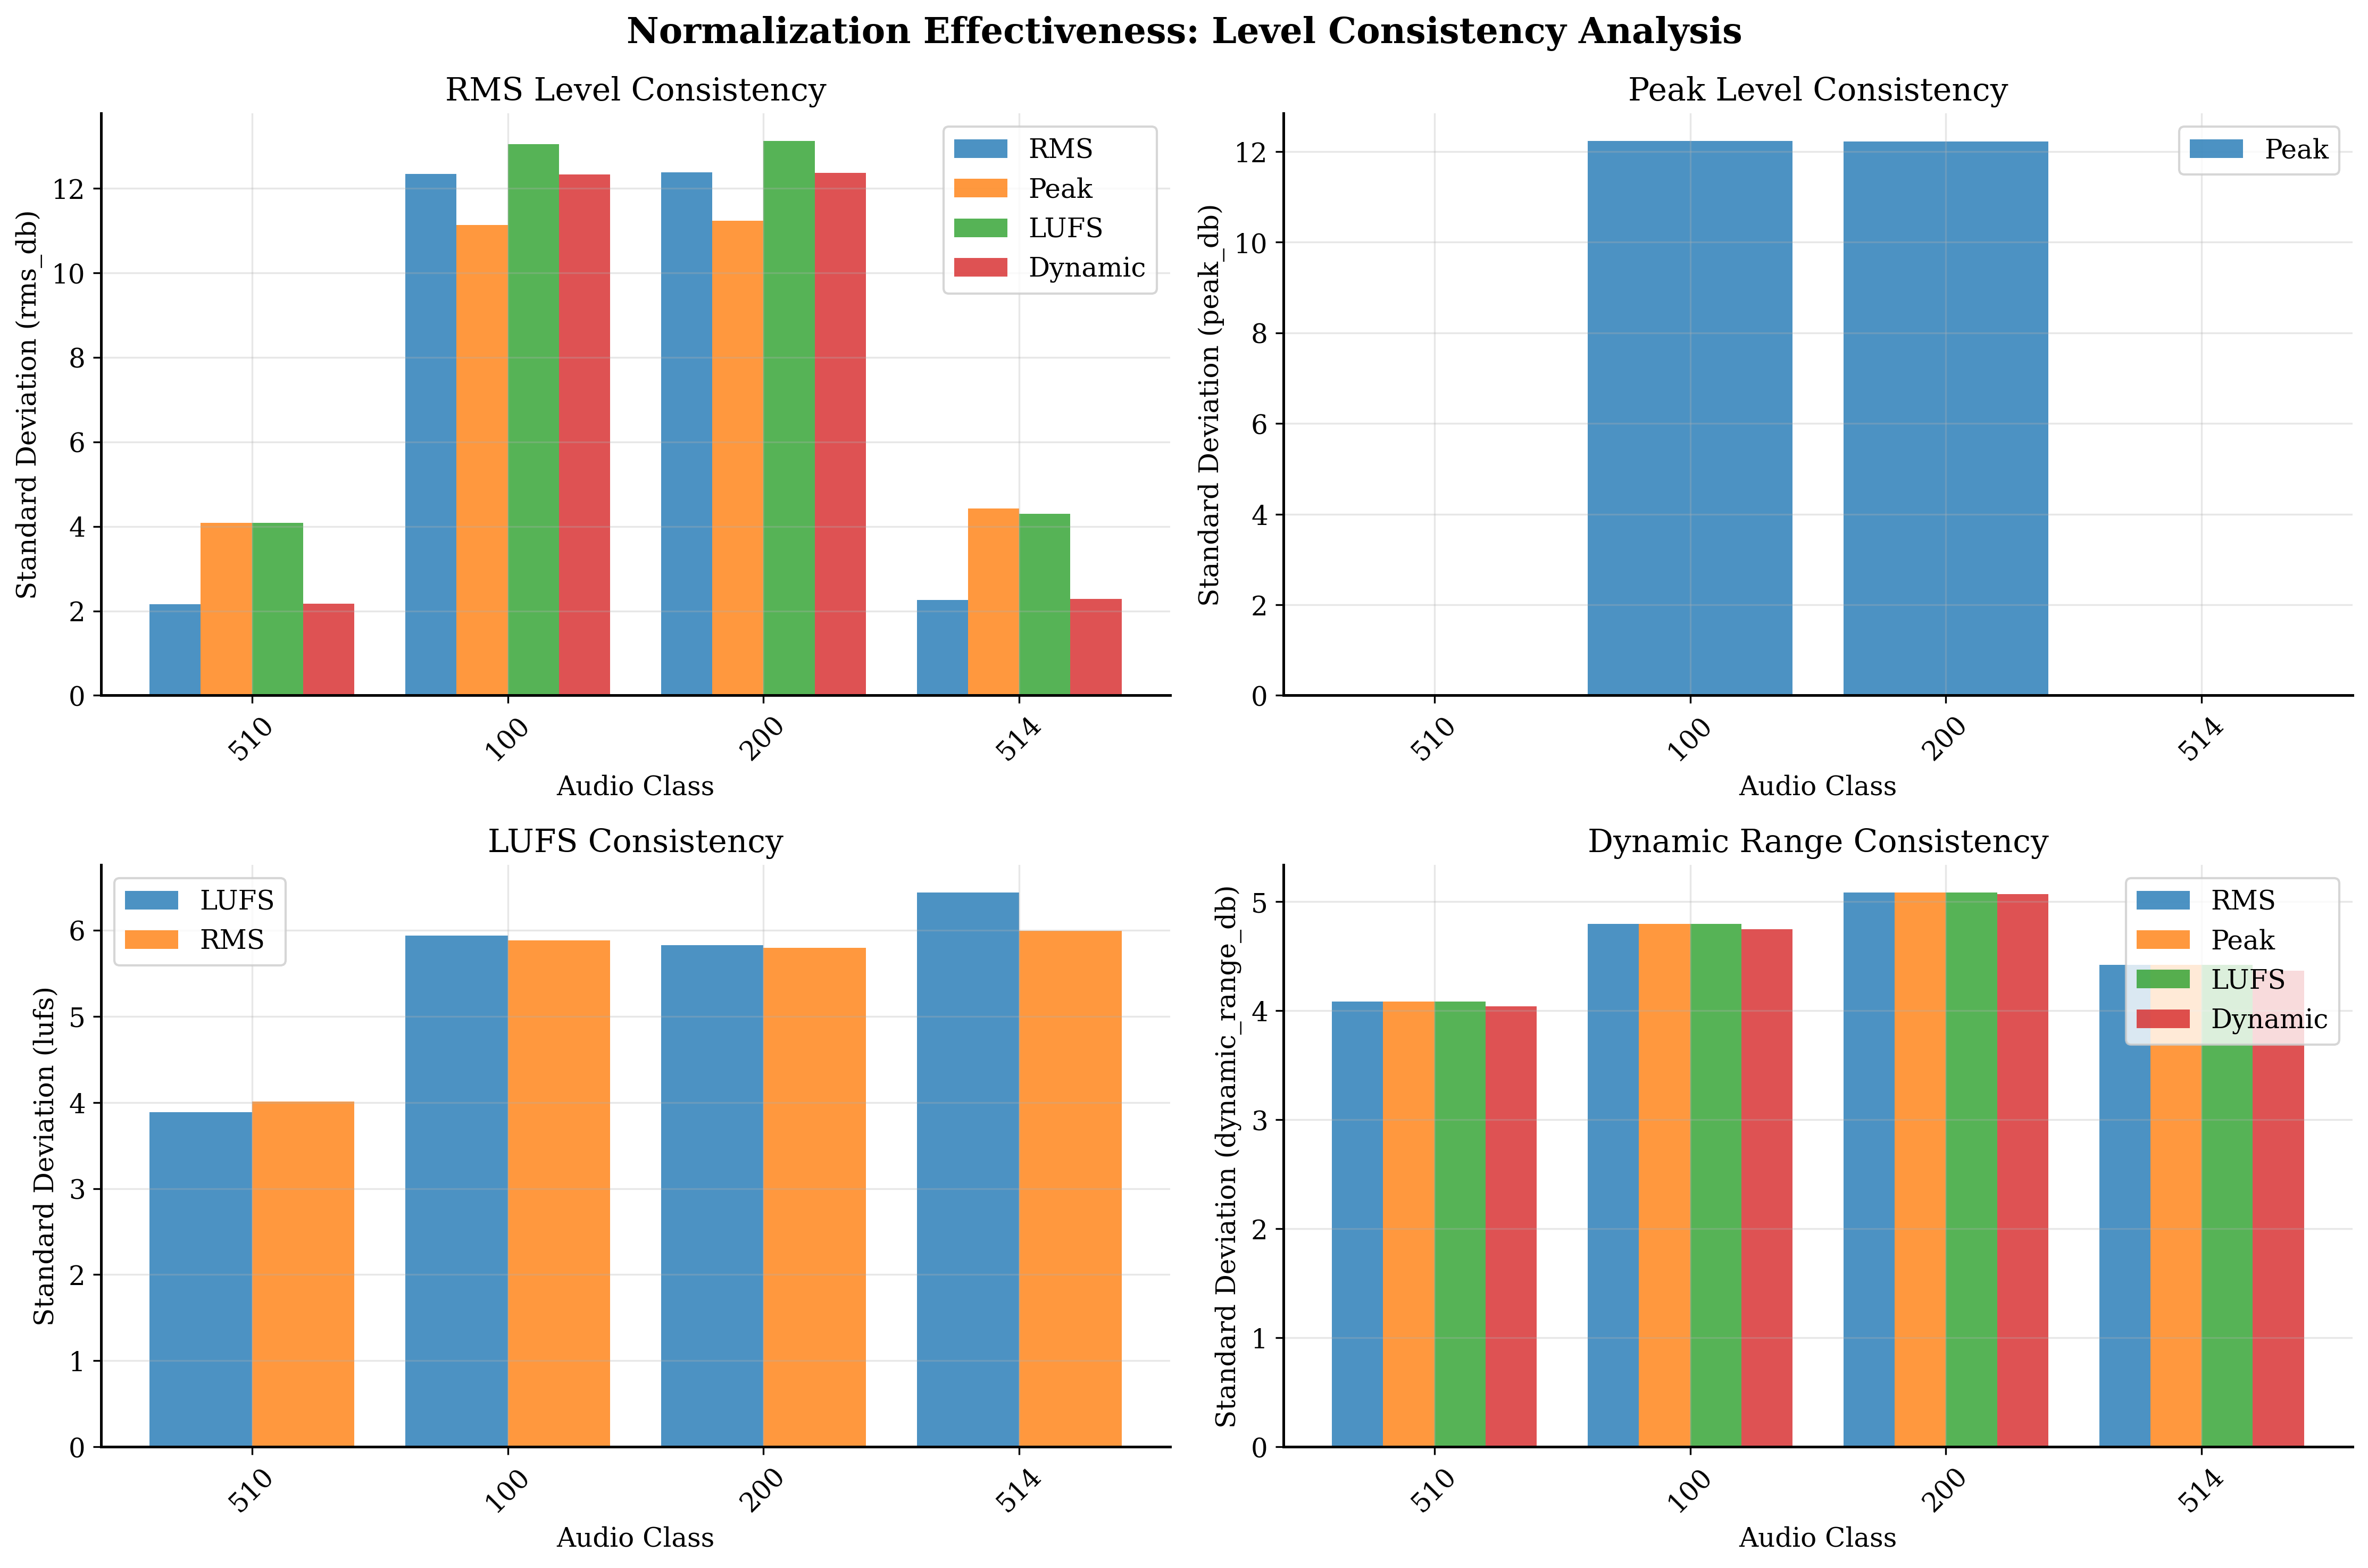
\includegraphics[width=\textwidth]{img/normalization_effectiveness.png}
    \caption{Effectiveness of the normalization process, showing the distribution of LUFS values before and after normalization.}
    \label{fig:norm_effectiveness}
\end{figure}

\section{Conclusion}
The described methodology provides a systematic and scientifically rigorous framework for the analysis and visualization of spatial audio. By decomposing binaural audio signals into their constituent time-frequency representations and subsequently computing a rich set of explicit binaural and spatial features, the software transforms the complex, time-varying signal into a comprehensive, multi-faceted representation. The inclusion of mathematical formulations for key algorithms such as the STFT, ILD, GCC-PHAT, and MSC solidifies the technical foundation of the approach. The results from the normalization analysis confirm the necessity and efficacy of the preprocessing stage, which ensures that subsequent feature extraction is performed on a consistent and comparable basis. The resulting feature mosaics are suitable for both qualitative analysis by researchers and as a direct input for quantitative analysis with modern machine learning models. The emphasis on standardized preprocessing, multi-resolution analysis, and the archiving of raw data ensures that the framework is robust, reproducible, and provides a powerful tool for research in spatial audio perception and technology.

\bibliographystyle{plainnat}
\bibliography{report}

\end{document}
